\documentclass[../../main.tex]{subfiles}

\begin{document}


\section{自定义简单宏}
论文中一般会频繁的出现一些较长的符号或专有名词,用简单的宏命令就可以方便的进行输入和全局修改。
这有点像C语言里面的宏,LaTeX编译器会使用命令中定义的文本内容代替实际的命令。

定义新的宏命令的方法:

\begin{verbatim}
\newcommand{commandName}[argumrntNum]{def}
\end{verbatim}

commandName是定义的新命令的名字,使用时以反斜线开头,区分大小写,可以使用汉字,
不能和LaTeX中自带的和模板中已经定义的命令名重复。

注意由于命令的名字可以是汉字,像
\begin{verbatim}
	\par一些文字
\end{verbatim}
这样的命令会出现“Undefined control sequence”错误,因为编译器将命令\verb|\par|后面的汉字也识别为变量名的一部分。为了避免这种情况,应该像
\begin{verbatim}
	\par 一些文字
\end{verbatim}
这样,用空格将命令和文本分开。

方括号中的arguumentNum是传入参数的个数,必须为数字,最大为9。如果不需要传参数,不写方括号即可。

def是宏的内容,传入的参数可以在内容中使用\verb|#1,#2,|$\cdots$,\verb|#9|来表示和区分。

简单的例子:

\begin{verbatim}
一个无参的例子:
\newcommand{vga}{VGA(Video Graphics Array)视频图形阵列}


2个参数的情况:
\newcommand{\ffield}[2]{有限域$\mathbf{\mathbb{#1}}_{#2}$}
命令的使用:
\ffield{F}{q}
\ffield{G}{a}

\end{verbatim}

产生的效果如下:
\newcommand{\ffield}[2]{有限域$\mathbf{\mathbb{#1}}_{#2}$}

\ffield{F}{q}

\ffield{G}{a}




建议把自定义的简单宏都放在导言区进行统一管理,不要到处乱放,以免造成混乱。
模板中提供的一些简单宏命令:

字体命令


\begin{figure}[htbp]
\centering

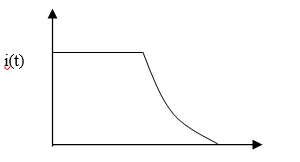
\includegraphics{../../figure/guozuni.png}
\caption{过阻尼响应}
\label{guozuni}
\end{figure}



\end{document}